{\textbf{1. 顺序存储}}

举2维数组的例子,同样是存储A{[}4{]}{[}5{]}中的9个元素:

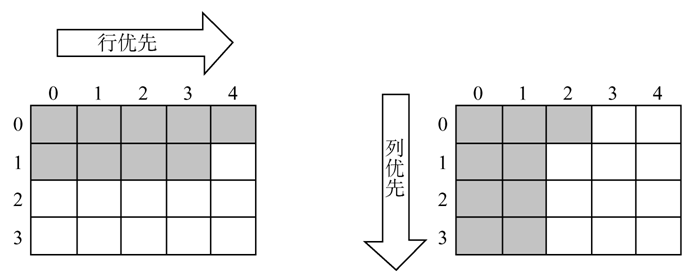
\includegraphics[width=3.12500in,height=1.22917in]{png-jpeg-pics/8C488ABCE9077951EA00275DDE50F718.png}

{a.
行优先连续存储的是A{[}0{]}{[}0~4{]}和A{[}1{]}{[}0~3{]}。}{列优先连续存储的是A{[}0~3{]}{[}0{]}、A{[}0~3{]}{[}1{]}和A{[}0{]}{[}2{]}。}

{b.
这里主要是涉及元素实际地址的计算。如给出A{[}0{]}{[}0{]}的地址求A{[}2{]}{[}3{]}的地址,在行优先和列优先就不同。}

{c.
在行优先的情况下,A{[}2{]}{[}3{]}为第14个元素,地址为A{[}0{]}{[}0{]}的地址加上13个元素空间的位移。}{在列优先的情况下,A{[}2{]}{[}3{]}为第15个元素,地址为A{[}0{]}{[}0{]}的地址加上14个元素空间的位移。}
